\documentclass[12pt, twoside]{article}
\usepackage[francais]{babel}
\usepackage[T1]{fontenc}
\usepackage[latin1]{inputenc}
\usepackage[left=5mm, right=5mm, top=2mm, bottom=2mm]{geometry}
\usepackage{float}
\usepackage{graphicx}
\usepackage{array}
\usepackage{multirow}
\usepackage{amsmath,amssymb,mathrsfs}
\usepackage{soul}
\usepackage{textcomp}
\usepackage{eurosym}
 \usepackage{variations}
\usepackage{tabvar}


\pagestyle{empty}

\begin{document}

\begin{center}
\textbf{\Large{Devoir maison 5}}
\end{center}


\enskip




\begin{center}
\fbox{

\textit{Devoir � rendre sur feuille grand format pour le
\textbf{mardi 18 mars 2014}. Devoir not� sur 30 points. }

}
\end{center}

\enskip

\begin{tabular}{cc}
\begin{minipage}{9cm}
\ul{Exercice 1:} \textit{(5,5 points)}

\enskip

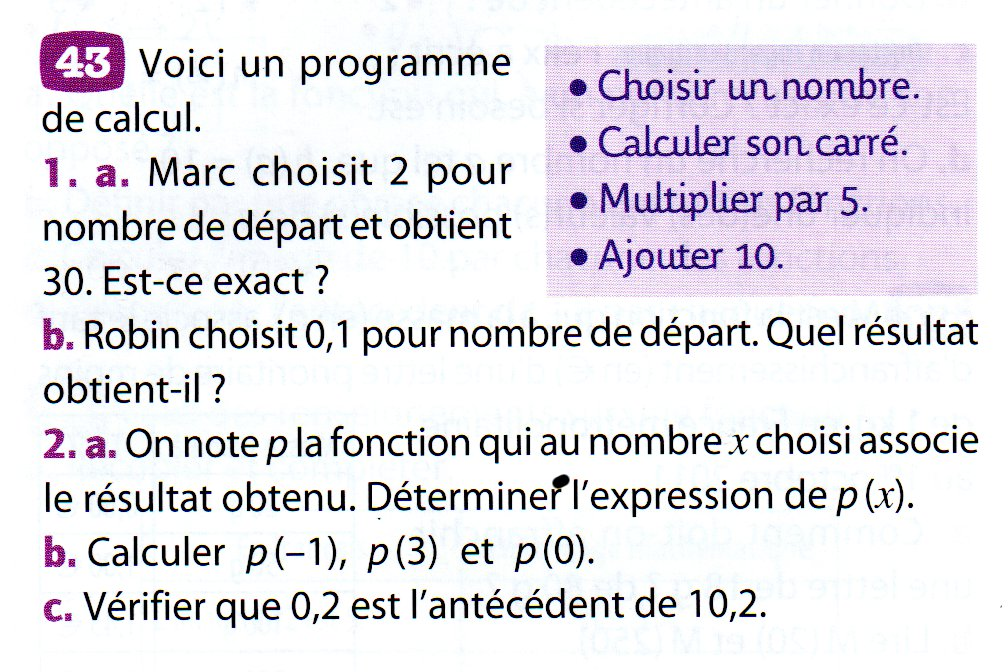
\includegraphics[width=8cm]{images/ex1.jpg}
\end{minipage}
&
\begin{minipage}{9cm}

\ul{Exercice 2:} \textit{(5 points)}

\enskip

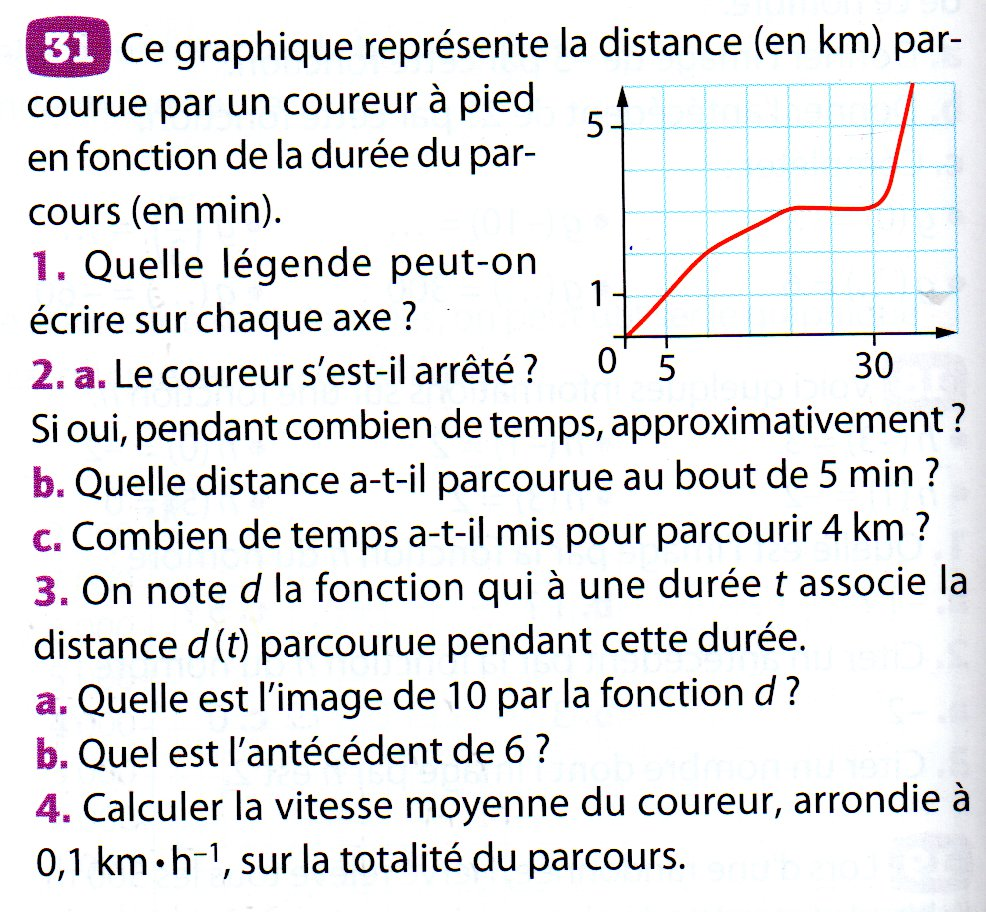
\includegraphics[width=8cm]{images/ex2.jpg}
\end{minipage}
\end{tabular}





\medskip

\begin{tabular}{cc}
\begin{minipage}{9cm}
\ul{Exercice 3:} \textit{(3 points)}

\enskip

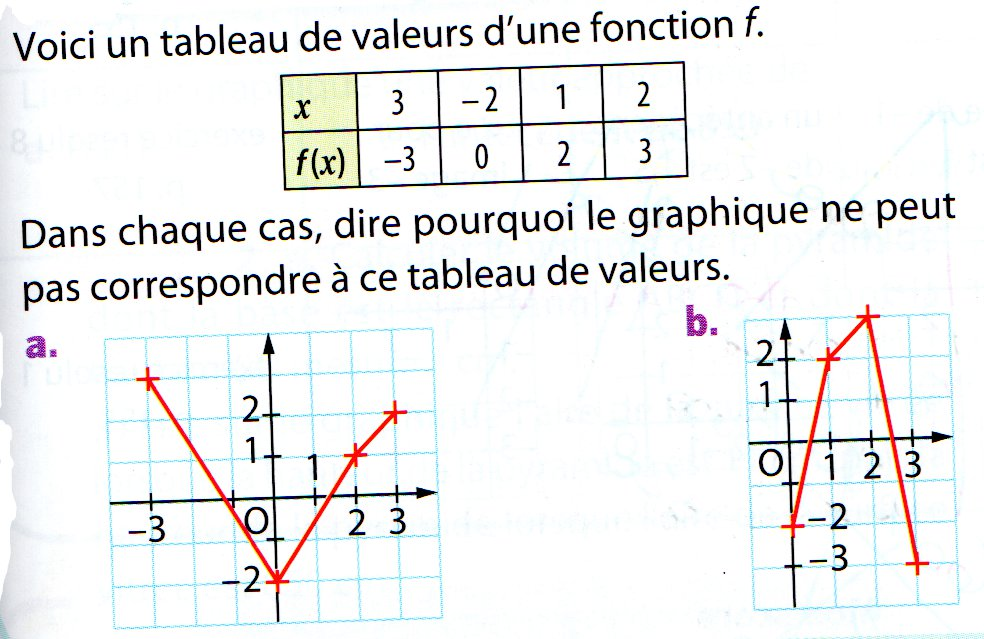
\includegraphics[width=8cm]{images/ex3.jpg}
\end{minipage}
&
\begin{minipage}{10cm}

\ul{Exercice 4:} \textit{(5 points)}

\enskip


\includegraphics[width=8cm]{images/ex4.png}



\end{minipage}
\end{tabular}


\bigskip


\ul{Exercice 5:} \textit{(4 points)}
\qquad \qquad 
$A=\dfrac{3 \times 10^5 \times 4 \times (10^{-3})^2}{16 \times 10^{-4}}$ \qquad
\qquad \qquad $B=\dfrac{7}{15}-\dfrac{2}{15} \times \dfrac{9}{4}$

\begin{enumerate}
  
  \item  Donner l'�criture d�cimale de A puis son �criture scientifique. Vous
  �crirez les diff�rentes �tapes de calcul.
  \item Calculer B et donner son r�sultat sous forme d'une fraction
  irr�ductible. Vous �crirez
  les diff�rentes �tapes de calcul.
 
\end{enumerate}
\bigskip

\ul{Exercice 6:} \textit{(3 points)}

\enskip

Dans la cour d'une ferme, il y a des poules, des moutons et un chien. Le nombre
de poules est �gal au tiers du nombre de moutons. Elsa a compt� les pattes et
en trouve 172. Combien y a-t-il de moutons et de poules?


\medskip

\ul{Exercice 7:} \textit{(4,5 points)}

\enskip


\begin{tabular}{cc}
\begin{minipage}{13cm}
\textit{Toutes les r�ponses doivent �tre justifi�es.}

\enskip

Des �l�ves participent � une course � pied. Avant l'�preuve, un plan leur a �t�
remis. Il est repr�sent� par la figure ci-contre.

\enskip

Sur cette figure, les droites (AE) et (BD) se coupent en C, les droites (AB) et
(DE) sont parall�les et ABC est un triangle rectangle en A.


Calculer la longueur r�elle du parcours ABCDE.

\end{minipage}
&
\begin{minipage}{6cm}

\begin{center}
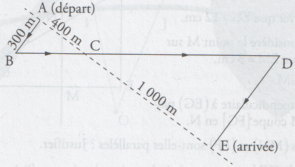
\includegraphics[width=6cm]{images/ex7.png}
\end{center}


\end{minipage}
\end{tabular}
 
\end{document}